\section{Integration Strategy}

\subsection{Entry Criteria}
Specify the criteria that must be met before integration testing of specific elements may begin (e.g., functions must have been unit tested).

\subsection{Elements to be integrated}
Identify the components to be integrated, refer to your design document to identify such components in a way that is consistent with your design.

\subsection{Integration Testing Strategy}
Describe the integration testing approach (top-­‐down, bottom-­‐up, functional groupings, etc.) and the rationale for the choosing that approach.

\subsection{Sequence of Component/Function Integration}
Depends on strategy chosen, this is a proposed structure.

\subsubsection{Software Integration Sequence}
For each subsystem, identify the sequence in which the software components will be integrated within the subsystem; relate this sequence to any product features that are being built up.

\paragraph{RentManager} 
The diagram above shows the needed precedences in the integration phase inside the \emph{RentManager} component.
\paragraph{}

		\begin{figure}[h]
			\centering
			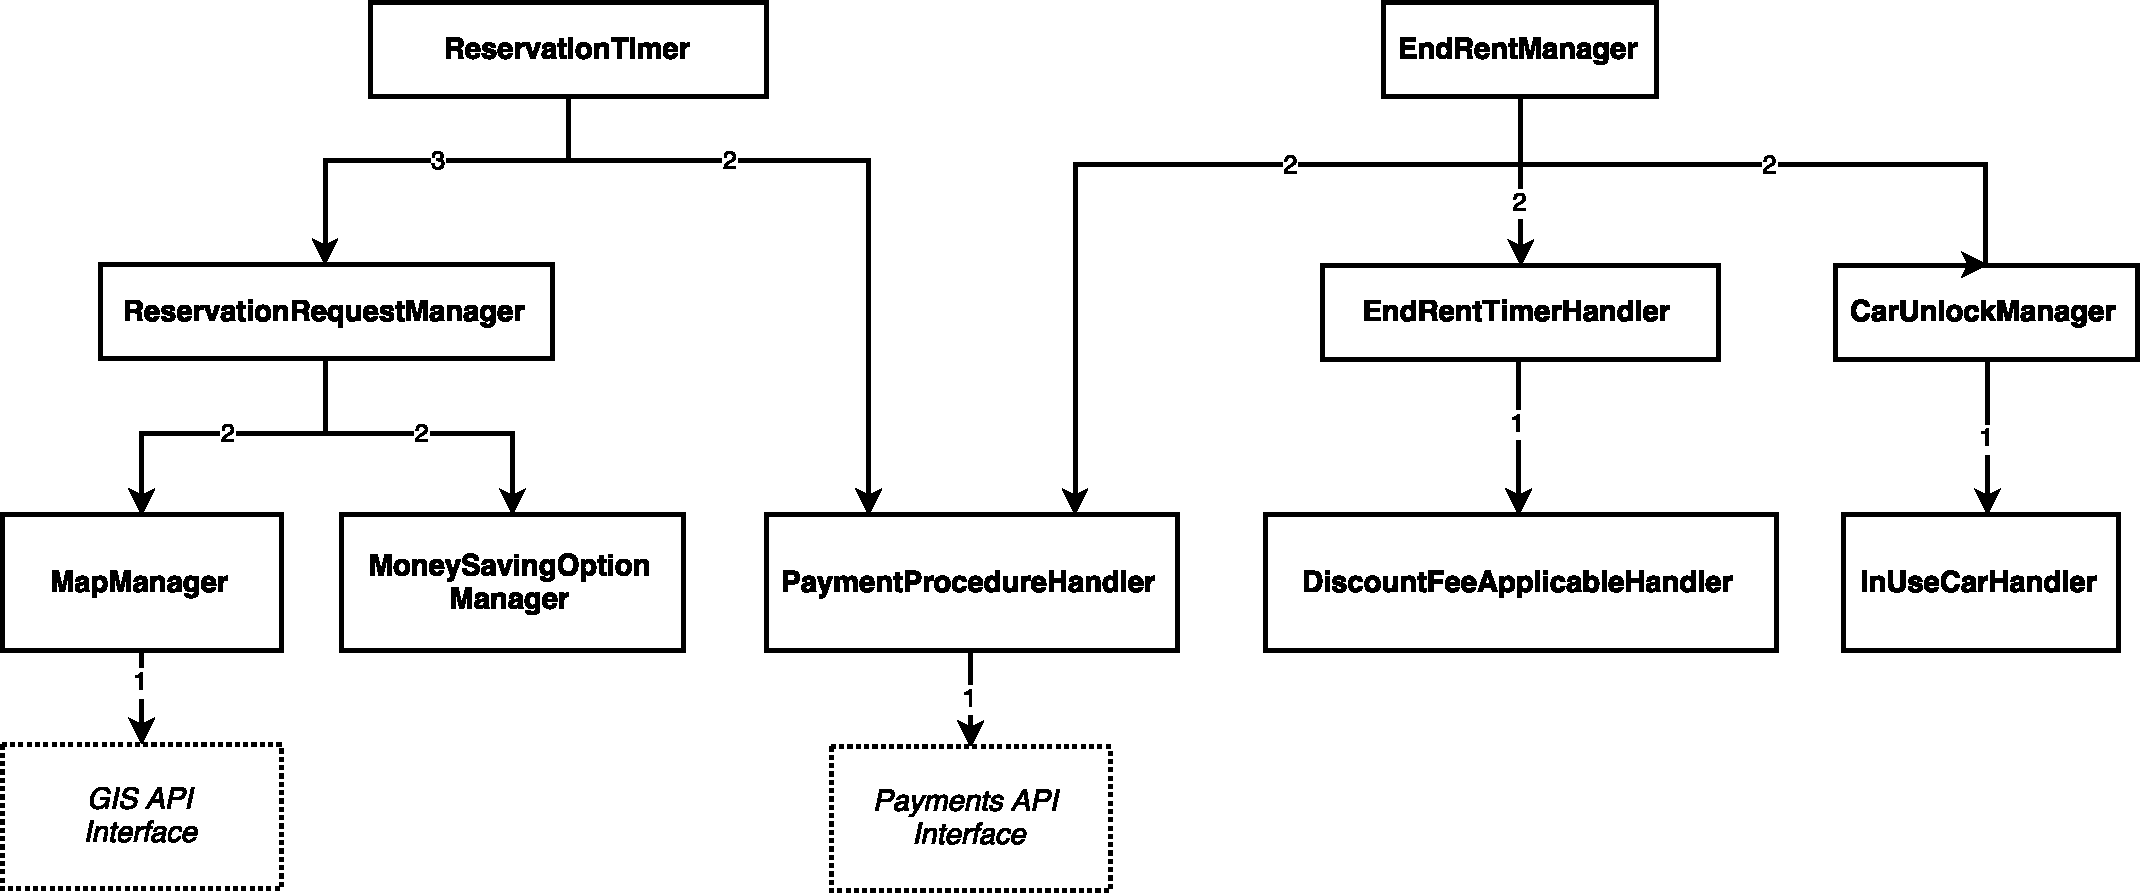
\includegraphics[width=\linewidth]{img/rentManagerIntegration}
			\caption{
				\label{fig:rentManagerIntegration} 
				\emph{RentManager integration}
			}
		\end{figure}
		
\paragraph{MaintenanceManager} 
The diagram above shows the needed precedences in the integration phase inside the \emph{MaintenanceManager} component.
\paragraph{}

		\begin{figure}[h]
			\centering
			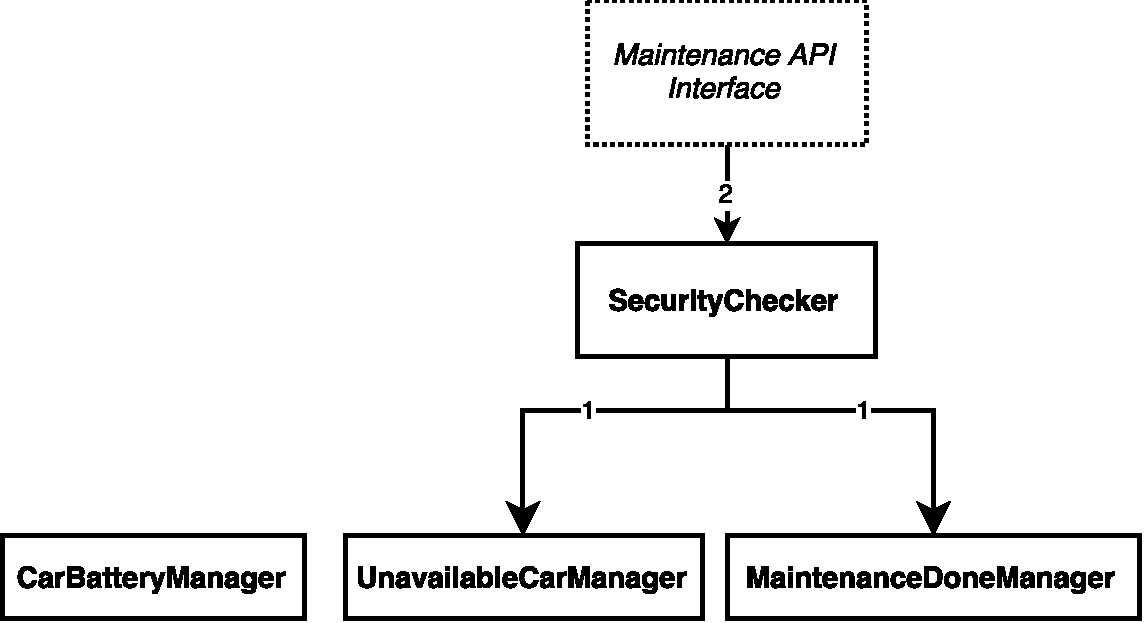
\includegraphics[width=\linewidth]{img/maintenanceIntegration}
			\caption{
				\label{fig:maintenanceIntegration} 
				\emph{MaintenanceManager integration}
			}
		\end{figure}
		
\paragraph{UserInformationManager} 
The diagram above shows the needed precedences in the integration phase inside the \emph{UserInformationManager} component.
\paragraph{}

		\begin{figure}[h]
			\centering
			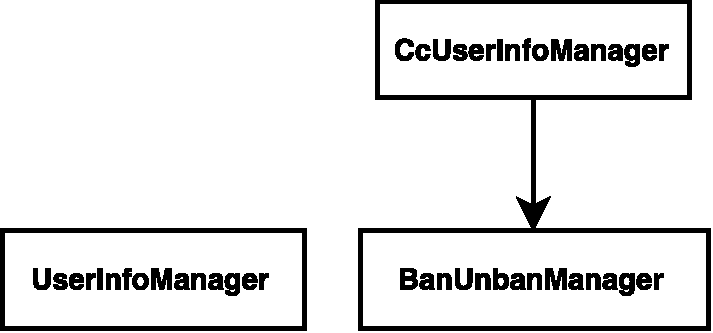
\includegraphics[width=0.6\linewidth]{img/userIntegration}
			\caption{
				\label{fig:userIntegration} 
				\emph{UserInformationManager integration}
			}
		\end{figure}

\subsubsection{Subsystem Integration Sequence}
Identify the order in which subsystems will be integrated; if you have a single subsystem, 2.4.1 and 2.4.2 are to be merged in a single section.
